\documentclass[border=4pt]{standalone}
\usepackage{tikz}
\usetikzlibrary{arrows.meta,positioning,shapes.geometric}

\begin{document}
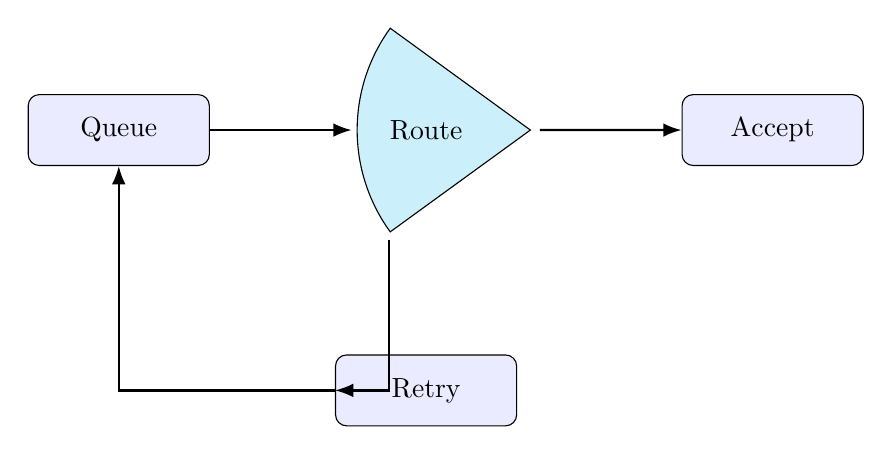
\begin{tikzpicture}[
  >=Latex,
  node distance=18mm,
  process/.style={draw,rounded corners,minimum width=23mm,minimum height=9mm,fill=blue!8},
  gate/.style={circular sector,circular sector angle=72,draw,fill=cyan!20,
    minimum width=28mm,minimum height=22mm,outer sep=2pt},
  flow/.style={->,thick}
]
  \node[process] (queue) {Queue};
  \node[gate,right=of queue] (route) {Route};
  \node[process,right=of route] (accept) {Accept};
  \node[process,below=of route] (retry) {Retry};

  \draw[flow] (queue) -- (route);
  \draw[flow] (route.sector center) -- (accept);
  \draw[flow] (route.arc end) |- (retry);
  \draw[flow] (retry.west) -| (queue.south);
\end{tikzpicture}
\end{document}
